\documentclass{article}
\usepackage{amsmath,amssymb}
\usepackage{tikz}
\usetikzlibrary{arrows.meta,positioning,calc,shapes.geometric}
\pagestyle{empty}
\begin{document}
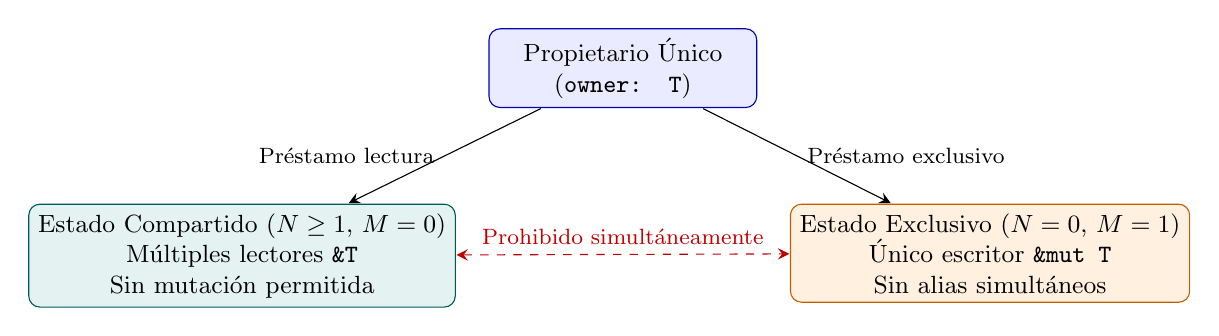
\begin{tikzpicture}
\tikzset{node distance=1.8cm, >=stealth, thick, font=\small}
\node[draw=blue!70!black, fill=blue!8, rounded corners, minimum width=3.4cm, minimum height=1.0cm, align=center] (own) {Propietario Único\\(\texttt{owner: T})};
\node[draw=teal!70!black, fill=teal!10, rounded corners, minimum width=4.2cm, minimum height=1.1cm, align=center, below left=1.2cm and 0.4cm of own] (imm) {Estado Compartido ($N \ge 1$, $M = 0$)\\Múltiples lectores \texttt{\&T}\\Sin mutación permitida};
\node[draw=orange!75!black, fill=orange!12, rounded corners, minimum width=4.2cm, minimum height=1.1cm, align=center, below right=1.2cm and 0.4cm of own] (mut) {Estado Exclusivo ($N = 0$, $M = 1$)\\Único escritor \texttt{\&mut T}\\Sin alias simultáneos};
\draw[->] (own) -- node[left, font=\footnotesize] {Préstamo lectura} (imm);
\draw[->] (own) -- node[right, font=\footnotesize] {Préstamo exclusivo} (mut);
\draw[<->, dashed, red!75!black] (imm) -- node[above, font=\footnotesize] {Prohibido simultáneamente} (mut);
\end{tikzpicture}
\end{document}
